\documentclass[12pt,DIV14,BCOR10mm,a4paper,parskip=half-,headsepline,headinclude,english,ngerman,bibliography=totocnumbered]{scrreprt}

\usepackage{hshhelper_base}

%%%%%%%%%%%%%%%%%%%%%%%%%%%%%%%%%%%%%%%%%%%%%%%%%%%%%%%%%%%%%%%%%%%%%%%%%%
\begin{document}    % hier gehts los
  \thispagestyle{empty} % Titelseite

\includegraphics[width=0.2\textwidth]{Wortmarke_WI_schwarz}

   {  ~ \sffamily
  \vfill
  {\Huge\bfseries Bedrohungsanalyse}
  \bigskip

  {\Large
  Dennis Grabowski, Julius Zint, Philip Matesanz, Torben Voltmer \\[2ex]
  Masterprojekt \enquote{Entwicklung und Analyse einer sicheren \\Web-Anwendung} \\
  Wintersemester 18/19
 \\[5ex]
   \today }
}
 \vfill

  ~ \hfill
  
\includegraphics[height=0.3\paperheight]{H_WI_Pantone1665}

\vspace*{-3cm}

\tableofcontents  % Inhaltsverzeichnis

\chapter{Zur Analyse verwendeten Methoden}
\section{Datenflussdiagramm}

Das folgende \gls{dfd} wurde mithilfe des Programms \enquote{OWASP Threat Dragon} \autocite{OWASP.ThreatDragon} erstellt.
Dieses Programm erlaubt leider keine Einfärbung in grün zur Kennzeichnung vertrauenswürdiger Prozesse oder Datenflüsse.
Alle schwarz gekennzeichneten Elemente sind daher als vertrauenswürdig zu betrachten.
Dieses DFD soll als Übersicht über alle vorhandenen Datenflüsse dienen, ohne dabei jeden Manager oder Controller seperat aufzulisten, da für diese der Datenfluss der selbe wäre.

\begin{figure}[htbp]
  \hspace*{-2.5cm}
  \label{overview-dfd-pic}
  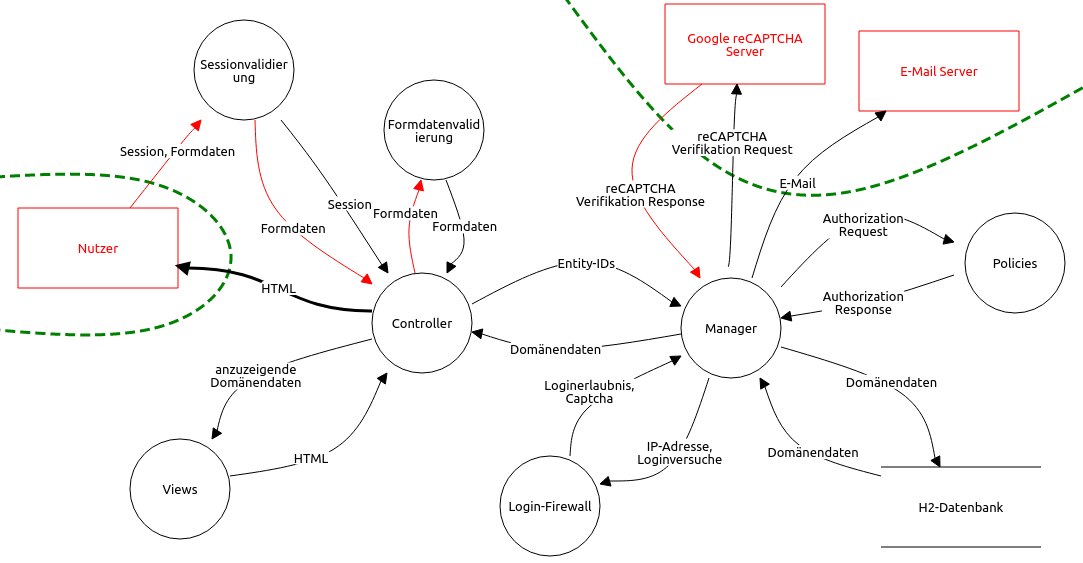
\includegraphics[width=1.25\linewidth]{resources/overview-dfd.jpg}
  \caption{Gesamtübersicht des Datenflusses in unserer Applikation}
\end{figure}

\subsection{Layered Entrypoints}

Die folgende Liste stellt alle vorhandenen Eintrittspunkte unserer Applikation in einer Baumstruktur vor.
Die Eintrittspunkte wurden für die bessere Übersicht nach \texttt{Controller} gruppiert, der für diesen Eintrittspunkt zuständig ist.
Zusätzlich werden die Parameter aufgelistet, die wir von dem Nutzer bei dem jeweiligen Eintrittspunkt entgegennehmen.
Sie dient hauptsächlich der Vollständigkeit und als Referenzliste, damit kein Eintrittspunkt übersehen werden kann.

\begin{enumerate}
  \item HTTP (Port 80)
  \begin{enumerate}
    \item \texttt{HomeController}
    \begin{enumerate}
      \item GET - \texttt{/}
    \end{enumerate}

 \item \texttt{LoginController}
    \begin{enumerate}
     \item \texttt{/login}
      \begin{enumerate}
        \item GET - \texttt{showLoginForm()}
        \item POST - \texttt{login(username, password, recaptcha)}
      \end{enumerate}
      \item \texttt{/logout}
      \begin{enumerate}
        \item POST - \texttt{logout()}
      \end{enumerate}
      \item \texttt{/changePasswordAfterReset}
      \begin{enumerate}
        \item GET - \texttt{showChangePasswordAfterResetForm}
        \item POST - \texttt{changePasswordAfterReset(username, currentPassword, password, passwordRepeat, recaptcha)}
      \end{enumerate}
    \end{enumerate}
    \item \texttt{UserController}
    \begin{enumerate}
      \item \texttt{/users}
      \begin{enumerate}
        \item GET - \texttt{showUsers()}
      \end{enumerate}
      \item \texttt{/users/create}
      \begin{enumerate}
        \item GET - \texttt{showCreateUserForm()}
        \item POST - \texttt{createUser(username, email)}
      \end{enumerate}
      \item \texttt{/users/delete}
      \begin{enumerate}
        \item POST - \texttt{deleteUser(userId)}
      \end{enumerate}
      \item \texttt{/resetpassword}
      \begin{enumerate}
        \item GET - \texttt{showResetUserPasswordForm}
        \item POST - \texttt{resetUserPassword(username)}
      \end{enumerate}
      \item \texttt{/sessions}
      \begin{enumerate}
        \item GET - \texttt{showActiveUserSessions()}
      \end{enumerate}
      \item \texttt{/sessions/delete}
      \begin{enumerate}
        \item POST - \texttt{deleteUserSession()}
      \end{enumerate}
    \end{enumerate}

    \item \texttt{GroupController}
    \begin{enumerate}
      \item \texttt{/user/groups}
      \begin{enumerate}
        \item GET - \texttt{showOwnGroups}
      \end{enumerate}
      \item \texttt{/groups}
      \begin{enumerate}
        \item GET - \texttt{showAllGroups}
      \end{enumerate}
      \item \texttt{/groups/create}
      \begin{enumerate}
        \item GET - \texttt{showCreateGroupForm}
        \item POST - \texttt{createGroup(groupname)}
      \end{enumerate}
      \item \texttt{/groups/:groupId}
      \begin{enumerate}
        \item GET - \texttt{showGroup(groupId)}
      \end{enumerate}
      \item \texttt{/groups/:groupId/members/remove}
      \begin{enumerate}
        \item POST - \texttt{removeGroupMember(groupId, userId)}
      \end{enumerate}
      \item \texttt{/groups/:groupId/members/add}
      \begin{enumerate}
        \item POST - \texttt{addGroupMember(groupId, userId)}
      \end{enumerate}
      \item \texttt{/groups/:groupId/delete}
      \begin{enumerate}
        \item POST - \texttt{deleteGroup(groupId)}
      \end{enumerate}
    \end{enumerate}
  \end{enumerate}
  \item SMTP (Port 587)
  \begin{enumerate}
    \item Versand der E-Mail für den Passwort-Reset
  \end{enumerate}
\end{enumerate}

\chapter{Bedrohungen}
\section{Gefundene Bedrohungen}

\subsection{Globale Bedrohungen}

\begin{itemize}

  \hypertarget{threat1}{}
  \item \textbf{T1: Spoofing des Servers}
  \begin{itemize}
  \item Zweck:
  	\begin{itemize}
  		\item Ausspähen von Anmeldedaten der Benutzer
  		\item Ausspähen von Dateien, die ein Benutzer beim Hsh-Helfer hochladen möchte
  	\end{itemize}
  \item Möglichkeiten:
  	\begin{itemize}
  		\item IP-Spoofing
  		\item DNS manipulieren
  	\end{itemize}
  \item Risiko: Mittel
  \item Gegenmaßnahmen: Authentifizierung des HsH-Helfer Servers durch Zertifikate (HTTPS mit HSTS)
  \end{itemize}

  \hypertarget{threat2}{}
  \item \textbf{T2: Eavesdropping}
  \begin{itemize}
  \item Zweck:
  	\begin{itemize}
  		\item Primär Ausspähen von Anmeldedaten der Benutzer
  		\item Grundsätzlich sind allen Daten (Gruppennamen etc.) Ziel
  		%\item Ausspähen von Dateien, die ein Benutzer bei HsH-Helfer hochlädt
  		%\item Ausspähen von Dateien, die ein Benutzer bei HsH-Helfer runterlädt
  	\end{itemize}
  \item Möglichkeiten: Man-in-the-Middle-Angriff
  \item Risiko: Mittel
  \item Gegenmaßnahmen: Verschlüsselung durch HTTPS mit HSTS oder SecureCookie
  \end{itemize}

  \hypertarget{threat3}{}
  \item \textbf{T3: Replayattacken}
  \begin{itemize}
  \item Zweck: Mehrfach-Ausführung geschützter Aktionen
  \item Möglichkeiten (Bezogen auf unsere Anwendung): Keine
  \item Risiko: Note
  \item Gegenmaßnahmen: HTTPS %/ CSRF-Token
  \end{itemize}

  \hypertarget{threat4}{}
  \item \textbf{T4: Tampering}
  \begin{itemize}
  \item Zweck:
  	\begin{itemize}
  		\item Ausführung von nicht intendierten Aktionen (z.B. Benutzer-Löschen abfangen und Ziel-User-Id manipulieren)
  		\item Server-Response manipulieren (z.B. bösartiges JavaScript einbauen)
	\end{itemize}
  \item Möglichkeiten: Leitung splicen und Man-In-The-Middle durchführen
  \item Risiko: Mittel
  \item Gegenmaßnahmen: HTTPS
  \end{itemize}

  \hypertarget{threat5}{}
  \item \textbf{T5: Verwendung eines gefälschten,von einer anerkannten Zertifizierungsstelle signierten Zertifikates}
  \begin{itemize}
  \item Zweck:
  	\begin{itemize}
  		\item Spoofing des Servers
  		\item Man-in-the-Middle-Angriffe
   \end{itemize}
  \item Möglichkeiten: Kontrolliert man eine anerkannten Zertifizierungsstelle, können gefälschte Zertifikate für die HsH-Helfer Domain ausgestellt werden. Für HsH-Helfer Benutzer ist das nicht sofort einsehbar\footnote{Bereits geschehen durch türkischen Geheimdienst: \url{https://arstechnica.com/information-technology/2013/01/turkish-government-agency-spoofed-google-certificate-accidentally/}}.
  \item Risiko: Gering
  \item Gegenmaßnahmen: HTTP Public Key Pinning (HPKP)
  \end{itemize}

  \hypertarget{threat6}{}
  \item \textbf{T6: XSS (Cross Site Scripting)}
  \begin{itemize}
  \item Zweck: Ausführung von JavaScript im HsH-Helfer Kontext eines Benutzers
  \item Möglichkeiten: Eingaben, die ausgegeben werden, ohne Eingabevalidierung oder Ausgabecodierung auszuführen
  \item Risiko: Hoch
  \item Gegenmaßnahmen:
	\begin{itemize}
		\item Eingabevalidierung (Kleinbuchstaben und Zahlen, valide E-Mail-Adressen)
		\item X-XSS-Protection (vgl. \ref{x:xss:protection})
		\item Content Security Policy (CSP) des Browsers aktivieren
		\item Alte Browser bzw Browser die CSP nicht können aussperren (s. Zusatzfrage) %TODO: Das ist nicht implementiert und vllt auch garnicht so einfach. Ggf einfach in Assumptions aufnehmen, dass nur Browser verwendet werden, die CSP unterstützen
		\item Ausgabecodierung
	\end{itemize}
  \end{itemize}

  \hypertarget{threat7}{}
  \item \textbf{T7: SQL Injection}
  \begin{itemize}
  \item Zweck: Unzulässiges Lesen und Schreiben von Datenbankinhalten
  \item Möglichkeiten: Inline-SQL Queries ohne Seperation of Data and Code
  \item Risiko: Hoch
  \item Gegenmaßnahmen:
  \begin{itemize}
    \item Die H2 Einstellung \texttt{ALLOW\_LITERALS=NONE} verwenden
    \item Nur PreparedStatements benutzen
    \item Eingabevalidierung
  \end{itemize}
  \end{itemize}

  \hypertarget{threat8}{}
  \item \textbf{T8: Offline Password Brute Forcing}
  \begin{itemize}
  \item Zweck: Durch SQL Injection erbeutete Hashes in Plaintext verwandeln
  \item Möglichkeiten: Rainbowtables
  \item Risiko: Gering
  \item Gegenmaßnahmen: Passwörter nur gehashed mit Salt speichern
  \end{itemize}

  \hypertarget{threat9}{}
  \item \textbf{T9: Cross-Site-Request-Forgery (CSRF)}
  \begin{itemize}
  \item Zweck: Benutzer dazu bringen Aktionen auszuführen, die sie nicht intendiert haben
  \item Möglichkeiten:
  \begin{itemize}
          \item Einen fremden Benutzer dazu bringen, sich selbst auszuloggen
          \item Einem Administrator einen Request unterjubeln, durch welchen er einen Nutzer erstellt
  \end{itemize}
  \item Risiko: Hoch
  \item Gegenmaßnahmen: CSRF-Tokens bei Requests prüfen
  \end{itemize}

  \hypertarget{threat10}{}
  \item \textbf{T10: Session fälschen (Bestimmte oder Irgendeine)}
  \begin{itemize}
  \item Zweck: Client spoofen um Aktionen auszuführen, für die der gespoofte Client autorisiert ist
  \item Möglichkeiten: Cookie fälschen
  \item Risiko: Hoch
  \item Gegenmaßnahmen:
  \begin{itemize}
    \item Signieren des Cookies durch privaten Schlüssel,
    \item Verwendung von UUID,
    \item Bindung der Session an IP-Adresse,
    \item Begrenzung der Lebenszeiten
  \end{itemize}
  \end{itemize}

  \hypertarget{threat11}{}
  \item \textbf{T11: Abstreitbarkeit illegaler Handlungen}
  \begin{itemize}
  \item Zweck: Anderen Nutzer in rechtliche Schwierigkeiten bringen
  \item Möglichkeiten: Eintragen illegaler Namen bei Benutzernamen oder Gruppenmane
  \item Risiko: Gering
  \item Gegenmaßnahmen: Logging von IP + Zeit, Action, User
  \end{itemize}

  \hypertarget{threat12}{}
  \item \textbf{T12: Nutzer kann eine ihm unerlaubte Operation durchführen}
  \begin{itemize}
  \item Zweck: Beispielsweise um einen Denial-of-Service-Angriff auf einen Nutzer durchzuführen
  \item Möglichkeiten: Beispielsweise Nutzer löscht andere Nutzer
  \item Risiko: Mittelmäßig - Hoch
  \item Gegenmaßnahmen: Authorization erzwingen und prüfen bei jeder Operation
  \end{itemize}

  \hypertarget{threat13}{}
  \item \textbf{T13: Captchas durch menschliche Akteure lösen lassen}
  \begin{itemize}
  \item Zweck: Brute-Forcing ermöglichen
  \item Möglichkeiten: 2captcha.com bietet diesen Service für 2.99\$ für 1000 reCAPTCHAs
  \item Risiko: Gering
  \item Gegenmaßnahmen: Zwei-Faktor-Authentisierung
  \end{itemize}

  \hypertarget{threat14}{}
  \item \textbf{T14: DDOS}
  \begin{itemize}
  \item Zweck: Verfügbarkeit der Anwendung beeinträchtigen
  \item Möglichkeiten: Botnetzwerk oder Booter-Service verwenden
  \item Risiko: Mittel
  \item Gegenmaßnahmen: Cloudflare/Incapsula/Akamai Secure Shield verwenden
  \end{itemize}

  %\item \textcolor{red}{Elevation of privilege -> Frage an Peine. ?}
\end{itemize}

\subsection{Domänenspezifische Bedrohungen}

\subsubsection{Mögliche Angriffe auf den Loginprozess}

\begin{itemize}

  \hypertarget{threat15}{}
  \item \textbf{T15: Überlanges PW beim Login eingeben}
  \begin{itemize}
  \item Zweck: DOS der Applikation
  \item Möglichkeiten: Durch überlange Passwörter eine ressourcenintensive Hash-Operation in Gang setzen
  \item Risiko: Hoch
  \item Gegenmaßnahmen:
  \begin{itemize}
  \item Passwort-Länge mittels Eingabevalidierung beschränken
  \item Verwendung von bcrypt (lässt nur 72 Zeichen lange Passwörter zu, Laufzeit ist für alle Längen von Eingaben konstant)
  \end{itemize}
\end{itemize}

  \hypertarget{threat16}{}
  \item \textbf{T16: Timing-Angriff auf Loginverhalten}
  \begin{itemize}
  \item Zweck: Herausfinden, ob ein Benutzer mit einem bestimmten Username existiert
  \item Möglichkeiten: Durch Messen der Antwortszeiten des Servers können Rückschlüsse darüber gezogen werden, welcher Code ausgeführt wurde (zB Hashing/DB-Zugriff)
  \item Risiko: Mittel
  \item Gegenmaßnahmen: Loginprozess für jeden Fall gleich ablaufen lassen
  \end{itemize}

  \hypertarget{threat17}{}
  \item \textbf{T17: Online Brute-Forcing}
  \begin{itemize}
  \item Zweck: Unautorisierter Zugriff auf ein fremdes Benutzerkonto
  \item Möglichkeiten: Beispielsweise durch Wörterbuchattacken
  \item Risiko: Hoch
  \item Gegenmaßnahmen:
  \begin{itemize}
      \item Login nur möglich, wenn Captcha gelöst wird
      \item IP Sperre bei auffälligem Verhalten
      \item Schwache Passworter verbieten
      \item Zwei-Factor-Authentisierung % TODO: Ist nicht implementiert und ggf auch nicht mal eben so gemacht
    \end{itemize}
  \end{itemize}
\end{itemize}

\subsubsection{Mögliche Angriffe auf den \enquote{Passwort zurücksetzen lassen}-Prozess}

\begin{itemize}
  \hypertarget{threat18}{}
  \item \textbf{T18: Nutzer permanent aus der Applikation ausschliessen}
  \begin{itemize}
  \item Zweck: Denial-of-Service-Angriff auf einen individuellen Nutzer
  \item Möglichkeiten: Wiederholtes Absenden des Request mit richtigen Nutzernamen generiert bei jedem Request ein neues temporäres Passwort. Selbst wenn der Benutzer das temporäre Passwort ändert, wird er es nicht schaffen sich anzumelden, da dann bereits die Generierung ein neues temporäres Passwort vom Angreifer erzwungen wurde.
  \item Risiko: Hoch
  \item Gegenmaßnahmen:
  \begin{itemize}
  \item Einbau eines Captchas
  \item Dem Benutzer einen Link schicken, der geöffnet werden muss, um den \enquote{Passwort ändern}-Prozess anzustoßen. Der Link muss einen geheimen Token beinhalten, der nur HsH-Helfer und dem Empfänger der E-Mail bekannt ist. Das temporäre Passwort wird erst generiert, sobald auf den Link geklickt wird
  \end{itemize}
\end{itemize}

  \hypertarget{threat19}{}
  \item \textbf{T19: Timing-Angriff auf Verhalten des Requests}
  \begin{itemize}
  \item Zweck: Herausfinden, ob ein Benutzer mit einem bestimmten Username existiert
  \item Möglichkeiten: Durch Messen der Antwortszeiten des Servers können Rückschlüsse darüber gezogen werden, welcher Code ausgeführt wurde (E-Mail-Versand)
  \item Risiko: Mittel
  \item Gegenmaßnahmen:
  \begin{itemize}
    \item \enquote{Passwort zurücksetzen lassen}-Prozess in konstanter Länge ablaufen lassen, ggf. durch Absenden einer E-Mail an eine Dummy-E-Mail-Adresse
    \item E-Mail-Versand asynchron durchführen
    \end{itemize}
  \end{itemize}

  \hypertarget{threat20}{}
  \item \textbf{T20: E-Mail Postfach des Nutzers fluten}
  \begin{itemize}
  \item Zweck: Verbrauch der vorhandenen Resourcen seines E-Mail-Kontos
  \item Möglichkeiten: Wiederholtes Absenden des Forms durch Angabe seines Nutzernamens
  \item Risiko: Hoch
  \item Gegenmaßnahmen: Nutzer muss Captcha lösen bevor Prozess angestoßen werden darf
  \end{itemize}
\end{itemize}

\subsubsection{Mögliche Angriffe auf den \enquote{Passwort ändern}-Prozess}

% This is subject to change if we implement the link-based mitigation
Da dieser Prozess dem Loginprozess gleich ist, treten hier die selben Lücken auf.
Um das Dokument kurz zu halten, listen wir diese nicht nochmal auf.

\subsubsection{Mögliche Angriffe beim Versand von E-Mails}
Der Angriffsvektor SMTP sollte ausweislich der Aufgabenstellung nicht betrachtet werden. Wir listen aus diesem Grund keine diesbezüglichen Bedrohungen.

\newcommand{\linktothreat}[2]{\texorpdfstring{\protect\hyperlink{#1}{#2}}{}}%

\section{Ignorierte Bedrohungen}
\subsection{Captchas durch menschliche Akteure lösen lassen}
Die Kosten für diese Dienstleistung machen sie unwirtschaftlich in Anbetracht unseres Applikationskontexts.

\subsection{HTTP bezogene Bedrohungen}
Die Bedrohungen \linktothreat{threat1}{T1}, \linktothreat{threat2}{T2}, \linktothreat{threat3}{T3}, \linktothreat{threat4}{T4}, \linktothreat{threat5}{T5} werden ignoriert.
Ausweislich der Aufgabenstellung sollen wir eine sichere Verbindung annehmen.

\section{Vorzunehmende Gegenmaßnahmen}

In der Tabelle \ref{threat-analysis:mitigation-table} können die Gegenmaßnahmen, die wir geplant haben umzusetzen, entnommen werden.

\begin{table*}[hbt!]
  \captionof{table}{Auflistung aller vorzunehmenden Gegenmaßnahmen mit Referenz auf Angriff, der verhindert/erschwert wird}
  \label{threat-analysis:mitigation-table}
  \begin{tabularx}{\linewidth}{
    |>{\hsize=0.8\hsize} X |
    >{\hsize=0.2\hsize} X |
  }
  \hline
  \textbf{Gegenmaßnahme} & \textbf{Angriff} \\ \hline
    Eingabevalidierung & \linktothreat{threat6}{T6}, \linktothreat{threat7}{T7}, \linktothreat{threat15}{T15} \\ \hline
    Ausgabecodierung & \linktothreat{threat6}{T6} \\ \hline
    PreparedStatements & \linktothreat{threat7}{T7} \\ \hline
    \texttt{ALLOW\_LITERALS=NONE} aktivieren & \linktothreat{threat7}{T7} \\ \hline
    Salt auf Passwörter anwenden & \linktothreat{threat8}{T8} \\ \hline
    Hinzufügen von CSRF-Token zu Formularen/Requests & \linktothreat{threat9}{T9} \\ \hline
    Cookies mit privaten Schlüssel signieren & \linktothreat{threat10}{T10}\\ \hline
    Session-ID im UUID-Format persistieren & \linktothreat{threat10}{T10}\\ \hline
    Session an IP-Adresse binden & \linktothreat{threat10}{T10}\\ \hline
    Session-Lebenszeit stark begrenzen & \linktothreat{threat10}{T10}\\ \hline
    Aktionen inkl User, IP-Adresse und Zeit loggen & \linktothreat{threat11}{T11}\\ \hline
    Zwei-Faktor-Authentisierung & \linktothreat{threat13}{T13}, \linktothreat{threat17}{T17}\\ \hline
    Cloudflare, Akamai Secure Shield, Incapsula verwenden & \linktothreat{threat14}{T14}\\ \hline
    bcrypt als Hashing-Algorithmus verwenden & \linktothreat{threat15}{T15} \\ \hline
    Operationen unter konstanter, gleichbleibender Laufzeit - auch bei unterschiedlichen Ausführungssträngen - ausführen & \linktothreat{threat16}{T16}, \linktothreat{threat19}{T19}\\ \hline
    Verbieten schwacher Passwörter & \linktothreat{threat17}{T17} \\ \hline
    Captcha zwischenschalten, um Massenrequests entgegenzuwirken & \linktothreat{threat17}{T17}, \linktothreat{threat18}{T18}, \linktothreat{threat20}{T20}\\ \hline
    IP-Adresse bei auffälligem Verhalten sperren & \linktothreat{threat17}{T17}\\ \hline
    Aussperrung alter Browserversionen & \linktothreat{threat6}{T6} \\ \hline
    \enquote{Content Security Policy}-Header nutzen & \linktothreat{threat6}{T6} \\ \hline
    \enquote{X-XSS-Protection}-Header nutzen & \linktothreat{threat6}{T6} \\ \hline
  \end{tabularx}
\end{table*}

\subsection{HTTP Header}

In der folgenden Liste werden verschiedene sicherheitsrelevante \enquote{HTTP Headers} beschrieben, die uns helfen, einige der Gegenmaßnahmen zu realisieren.
Diese Werte werden empfohlen, um die \enquote{maximale} Sicherheit zu garantieren.
Entnommen haben wir diese Empfehlungen verschiedenen Seiten, darunter der \enquote{Mozilla's Enterprise Information Security}-Blog \autocite{Mozilla.SecureHeaders} und das \enquote{OWASP Secure Headers Project} \autocite{OWASP.SecureHeaders}, die wir beide als vertrauenswürdig betrachten.

\subsection{Referrer-Policy}
\begin{sloppypar}
\texttt{Referrer-Policy: origin-when-cross-origin, strict-origin-when-cross-origin}
\end{sloppypar}
Mit diesem Header kann gesteuert werden, welche Informationen als \enquote{Referrer} an die nächste besuchte Seite weitergegeben werden. \texttt{strict-origin-when-cross-origin} sorgt dafür, dass innerhalb der Seite die vollständige URL weitergegeben wird. Beim Besuchen einer anderen Seite wird nur die Domain weitergegeben. Wird dabei jedoch von HTTPS auf HTTP gewechselt, ist das Weitergeben jeder Information untersagt.

\subsection{X-Frame-Options}
\begin{sloppypar}
\texttt{X-Frame-Options: DENY}
\end{sloppypar}
Um zu verhindern, dass unsere Seite in einem \texttt{<frame>}, \texttt{<iframe>} oder \texttt{<object>} Element auf einer anderen Seite eingebettet wird, kann der Header \texttt{X-Frame-Options} verwendet werden. So kann Clickjacking verhindert werden. %So können \enquote{Clickjacking} sowie \texttt{<iframe>}-basierte CSRF-Angriffe verhindert werden.

\subsection{X-XSS-Protection}
\label{x:xss:protection}
\begin{sloppypar}
\texttt{X-XSS-Protection: 1; mode=block}
\end{sloppypar}
Durch den Header \texttt{X-XSS-Protection} wird der Browser angewiesen, eine XSS Erkennung zu versuchen. Dieses Feature ist für älteren Browser interessant, die noch kein CSP implementieren. Durch den Modus \enquote{block} wird das Laden der Seite abgebrochen, sobald ein XSS Versuch erkannt wird.

\subsection{X-Content-Type-Options}
\begin{sloppypar}
\texttt{X-Content-Type-Options: nosniff}
\end{sloppypar}
Mit diesem Header wird dem Browser verboten, \enquote{MIME sniffing}\footnote{Beim \enquote{MIME sniffing} versucht der Browser den richtigen MIME Type durch Betrachtung des Inhalts zu erraten, wenn er annimmt, dass der im \texttt{Content-Type} übermittelte Wert nicht korrekt ist.} zu betreiben. Er wird gezwungen den MIME Typ zu verwenden, der im \texttt{Content-Type} Header angegeben wurde.

\subsection{Content-Security-Policy}
\begin{sloppypar}
\texttt{Content-Security-Policy: default-src 'self'; script-src https://www.google.com/recaptcha/ https://www.gstatic.com/recaptcha/; frame-src https://www.google.com/recaptcha/}
\end{sloppypar}
Innerhalb diesem Header ist es möglich Richtlinien zu definieren, die den Zugriff auf verschiedene Resourcen kontrollieren.
Dadurch kann verhindert werden, dass JavaScript nicht von jeder URL geladen und ausgeführt werden darf, von welchen Quellen Bilder geladen werden dürfen, oder welches CSS eingebunden werden darf.
Dieser Header ist dem \enquote{X-XSS-Protection}-Header vorzuziehen.

%\subsection{X-Permitted-Cross-Domain-Policies}
%\begin{sloppypar}
%\texttt{X-Permitted-Cross-Domain-Policies: master-only}
%\end{sloppypar}

\printbibliography

% Can be used to add a list of acronyms with their description
%\glsaddall
%\deftranslation{to=German}{Acronyms}{Abkürzungsverzeichnis}
%\deftranslation{to=German}{Glossary}{Glossar}
\printacronyms[title=Abkürzungsverzeichnis,toctitle=Abkürzungsverzeichnis]
\printglossary[type=main]

%\addcontentsline{toc}{chapter}{\listfigurename}
\listoffigures      % Abbildungsverzeichnis

%s\addcontentsline{toc}{chapter}{\listtablename}
% \listoftables       % Tabellenverzeichnis

\end{document}
